%%%%%%%%%%%%%%%%%%%%
%
% $Beschreibung: Hier werden alle offenen Punkte, bis zum Abschluss des Projekts gesammelt $
% $Autor: ter Veen, Theilmann $
% $Datum: 09.06.2024 $
% $Pfad: DemonstratorSchrittmotor/DeveloperDoc/Contents/de/OffenePunkte.tex $
% $Version: 2 $
%
%
%%%%%%%%%%%%%%%%%%%

\chapter{Offene Punkte}

Dieses Projekt befindet sich noch in der Entwicklungsphase. Bei dem Demonstrator handelt es sich um ein Prototyp und es bietet noch an Verbesserungs- und Erweiterungspotenzial. In diesem Fall findet ausschließlich ein Ausblick zu Lern- und Demonstrationszwecken statt. 

\section{Misslungene Messung der Beschleunigung des Schlittens}

Zunächst sollte die Beschleunigung gemessen werden. Um die Beschleunigung des Schlittens zu messen, muss auf den Schlitten ein Beschleunigungssensor integriert werden. Dafür wurde ein Arduino Nano 33 Ble Sense Rev2 verwendet, der die gleiche 9-Achs-IMU (LSM9DS1) verwendet wie die im Arduino Nano 33 BLE Sense Lite. Die 9-Achs-IMU wird in Kapitel \ref{9Achs} genauer erläutert. Für die Befestigung des Arduinos wurde eine Konstruktion aus einem älteren Projekt verwendet, dabei handelt es sich um ein kleines Gehäuse indem der Arduino reingelegt wird und mit einer DIN 912 M3 Schraube an dem Schlitten befestigt wurde, zu sehen in Abbildung \ref{ArdRev2Schlitten}.

\begin{figure}[H]
	\begin{center}
		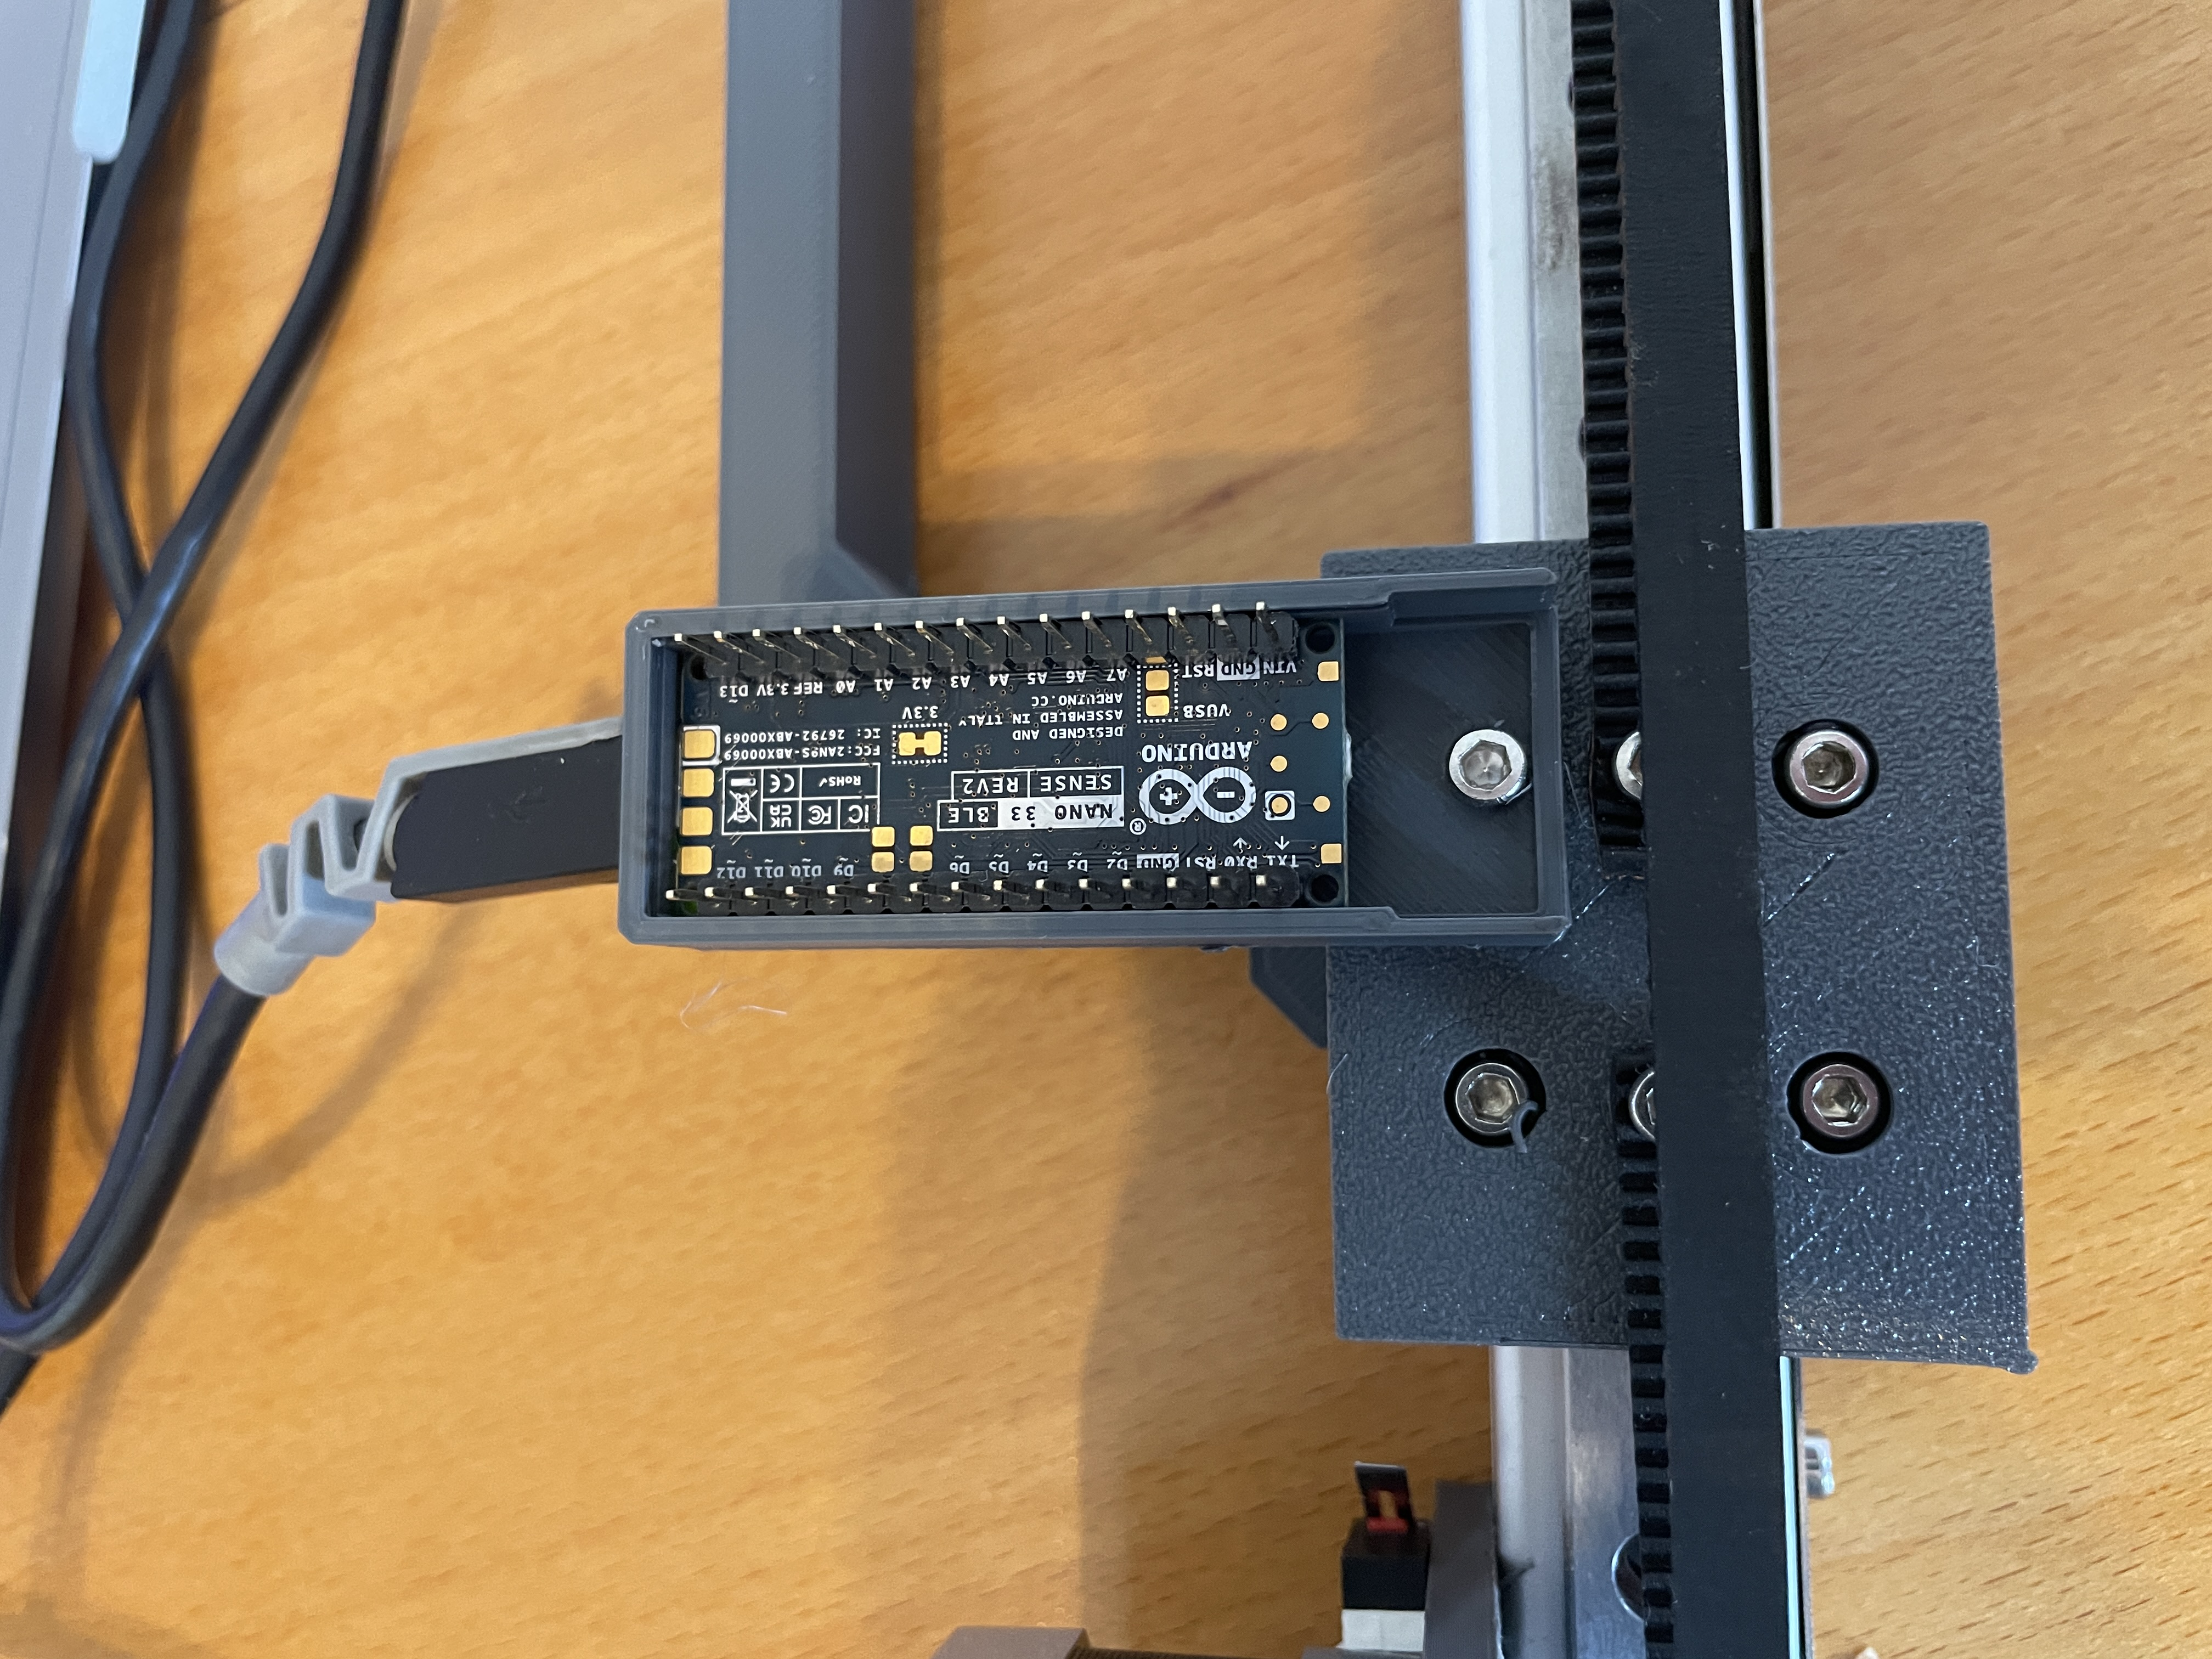
\includegraphics[width=\textwidth]{Images/Tests/ArdRev2Schlitten.jpg}
		\caption{Montage des Arduino Nano 33 Ble Sense Rev2 auf dem Schlitten} \label{ArdRev2Schlitten}
	\end{center}
\end{figure} 

Der notwendige Code für den Arduino lieferte die IDE mithilfe der Bibliothek ArduinoLSM9DS1 unter dem Pfad File/Examples/ArduinoLSM9DS1/SimpleAccelerometer. Der Code wurde lediglich an das Ausgeben der wichtigen Achse und die Umrechnung in m/s$^2$ angepasst. Der Messaufbau wird in Abbildung \ref{TestAuffbauACC} dargestellt. 

\begin{figure}[H]
	\begin{center}
		\includegraphics[width=\textwidth]{Images/Tests/TestAufbauACC.jpg}
		\caption{Testaufbau Messung Beschleunigung} \label{TestAuffbauACC}
	\end{center}
	\end{figure} 

Bei der Auswertung jedoch fiel auf, das obwohl mit verschiedenen eingestellten aber auch ersichtlichen Beschleunigungswerten oft der identische Wert angezeigt wurde. Es wurde dabei vermutet, dass durch die Vibrationen und die Eigenfrequenz des Systems es zu Ausreißern kommt. Zunächst wurde das Gehäuse demontiert, ergab keine Abhilfe. Der nächste Schritt war einen Filter gegen Ausreißer in dem Code einzupflegen, allerdings auch ohne Erfolg. 
Aus zeitlichen Gründen wurden die Bewegungsprofile in jeder Stufe auf die gleiche Beschleunigung angepasst. Unterschieden wird nur in den Geschwindigkeiten, sodass bei den Test ausschließlich die Messung der mittleren Geschwindigkeit durchgeführt werden konnte.    

\section{Misslungene Ansteuerung der SMD-LED}

Die Funktion der SMD-LED wurde im Test nachgewiesen und gab alle geforderten Farben aus. Die LED sollte die drei verschieden Demonstrator-Status anzeigen (Grün = Bereit für den Demonstrierablauf, Gelb = Referenzfahrt, Blau = Demonstrierablauf). Aufgrund mangelnder Digitalanschlüsse konnte nur die Farbe Rot ausgegeben werden, diese nun den Status anzeigt, dass das System allgemein bereit ist.  

\section{Verbesserungen}

Am offensichtlichsten ist die Überarbeitung des Gehäuses. Durch die Vibration des Motors wird häufig in die Eigenfrequenzen des Gehäuses gefahren, sodass eine starke Geräuschkulisse entsteht. Ein Spritzguss-Gehäuse mit verbesserte Konstruktion mit zum Beispiel eine Integration von elastischen Gehäusefüßen könnten diesen Mangel umgehen. Außerdem könnte weitere Einzelteile mit anderen Fertigungstechniken hergestellt werden um bessere Qualitäten der Bauteile zu erreichen.

Softwaretechnisch könnte ein verbesserter Code zu kürzeren Rechenzeiten des Prozessors und einen stabileren Lauf führen. Außerdem könnten die Bewegungsstufen besser und genau definiert werden um noch bessere Ergebnisse zu erzielen.   


\section{Erweiterung}

Die einfachste Erweiterung sind die Integration von neuen Bewegungsstufen per Software. Darüber hinaus könnte per Drehknopf eine manuelle Eingabe einer Geschwindigkeit und Beschleunigung oder ein Erreichen eines genauen Punktes hinzugefügt werden. Ein Integrieren eines Beschleunigungssensor auf dem Schlitten könnte zur genaueren Stufen führen indem das System durch den Sensor und einem Regler geregelt werden könnte. Des Weitere könnten Differenzen zwischen Eingabe und tatsächlichen Werten am OLED-Display angezeigt werden. 

\section{Anwendung in der Lehre}

Der Demonstrator kann durch die Kompakte Bauweise mobil mitgenommen und schnell aufgebaut werden. So kann der Demonstrator Studierende praktische Erfahrungen in verschieden Fachbereichen vermitteln. Die Fachrichten sind Automatisierungstechnik, Elektrotechnik, Steuerungstechnik, Maschinenelemente und viele mehr. Durch das Durchfahren der Stufen werden reale Situation von Schrittmotoren simuliert. Dies kann Einblicke in Anforderungen und Abläufe in der Industrie zeigen. 
